\documentclass[12pt]{article}

%--------------------------------------------------------------------
% PAGE & FONT SETUP
%--------------------------------------------------------------------
\usepackage[T1]{fontenc}
\usepackage[margin=1in]{geometry}
\usepackage{lmodern}         % Clean, modern font
\usepackage{ragged2e}        % Better text justification
\setlength{\parskip}{6pt}    % Space between paragraphs
\setlength{\parindent}{0pt}  % No paragraph indent

%--------------------------------------------------------------------
% COLORS & SECTION STYLING
%--------------------------------------------------------------------
\usepackage{xcolor}
\usepackage{sectsty}
\usepackage{titlesec}

% A cohesive, modern color palette:
\definecolor{mainDark}{HTML}{2C3E50}  % Deep blue-gray
\definecolor{mainLight}{HTML}{ECF0F1} % Light gray background
\definecolor{accentColor}{HTML}{3498DB} % Soft blue accent
\definecolor{boxBg}{HTML}{F8F9FA}    % Slightly off-white box background

% Section title color & spacing
\sectionfont{\color{mainDark}\huge}
\subsectionfont{\color{mainDark}\Large}
\subsubsectionfont{\color{mainDark}\large}

% Customize section title spacing
\titlespacing*{\section}{0pt}{0.8em}{0.5em}
\titlespacing*{\subsection}{0pt}{0.7em}{0.4em}

%--------------------------------------------------------------------
% HYPERLINKS
%--------------------------------------------------------------------
\usepackage{hyperref}
\hypersetup{%
  colorlinks=true,
  linkcolor=accentColor,
  urlcolor=accentColor
}

%--------------------------------------------------------------------
% CODE LISTINGS (MINTED)
%--------------------------------------------------------------------
\usepackage{minted}
\usemintedstyle{friendly} % Colorful, easy-to-read code style

%--------------------------------------------------------------------
% TIKZ FOR DIAGRAMS
%--------------------------------------------------------------------
\usepackage{tikz}
\usetikzlibrary{shapes,arrows,positioning,calc,arrows.meta,shapes.misc}

% Our custom TikZ styles, updated to match the new palette:
\tikzset{%
  serviceBox/.style={%
    rectangle,
    rounded corners,
    draw=mainDark,
    fill=boxBg,
    text width=2.8cm,
    minimum height=1.2cm,
    align=center
  },
  arrowLine/.style={%
    -{Latex[length=3mm,width=2mm]},
    thick,
    color=mainDark
  },
  cloudService/.style={%
    cloud,
    draw=mainDark,
    fill=boxBg,
    cloud puffs=15,
    cloud puff arc=120,
    aspect=2,
    minimum width=2.4cm,
    align=center
  },
  database/.style={%
    cylinder,
    cylinder uses custom fill,
    cylinder body fill=boxBg,
    cylinder end fill=boxBg,
    draw=mainDark,
    shape aspect=0.7,
    minimum height=2.2cm,
    minimum width=1.4cm,
    align=center
  },
  userFigure/.style={%
    rectangle,
    rounded corners,
    draw=mainDark,
    fill=green!15,
    text width=2.5cm,
    minimum height=1.1cm,
    align=center
  }
}

%--------------------------------------------------------------------
% TITLE
%--------------------------------------------------------------------
\title{%
  \vspace{-1.5cm}
  \color{mainDark}\Huge A Modern, Visual Introduction to AWS \\
  \vspace{0.1cm}
  \large \textit{(Beginner-Friendly Edition)}
}
\author{}
\date{}

\begin{document}
\maketitle

\thispagestyle{empty}
\vfill
\begin{center}
    \textit{\color{mainDark}
        This guide introduces core AWS concepts using diagrams and
        straightforward explanations. Ideal for newcomers seeking a
        quick yet clear jump into cloud computing.
    }
\end{center}
\vfill
\clearpage

%--------------------------------------------------------------------
% TABLE OF CONTENTS
%--------------------------------------------------------------------
\tableofcontents
\clearpage

%--------------------------------------------------------------------
% INTRO
%--------------------------------------------------------------------
\section*{Introduction}
\addcontentsline{toc}{section}{Introduction}
\justifying

\textbf{Amazon Web Services (AWS)} makes it easy to “rent” computing resources over the internet. Rather than buying and maintaining physical servers, you pay only for what you use. This document focuses on the essential building blocks of AWS, shown with easy-to-follow diagrams, so that by the end, you’ll have a clear picture of how to start.

\clearpage

%--------------------------------------------------------------------
% 1. WHAT IS AWS?
%--------------------------------------------------------------------
\section{What is AWS?}
\justifying

\subsection{High-Level Definition}
AWS is a \textbf{cloud computing} platform from Amazon. You can:
\begin{itemize}
    \item \textbf{Store data} (files, images, backups) reliably.
    \item \textbf{Run applications} (web, mobile, API services).
    \item \textbf{Analyze data and use AI} without building physical servers.
\end{itemize}

\textbf{Key Benefits}:
\begin{itemize}
    \item \textbf{Pay-As-You-Go}: No big upfront server costs.
    \item \textbf{Scalable}: Quickly handle growth (or traffic spikes).
    \item \textbf{Global Reach}: Deploy in many geographical regions.
\end{itemize}

\subsection{Core Service Areas}
\begin{itemize}
    \item \textbf{Compute}: EC2 (virtual servers), Lambda (serverless).
    \item \textbf{Storage}: S3 (object storage), EBS (attachable storage).
    \item \textbf{Databases}: RDS (relational), DynamoDB (NoSQL).
    \item \textbf{Networking}: VPC (private networks), CloudFront (CDN).
    \item \textbf{Analytics}: Kinesis (stream data), Athena (SQL on S3).
    \item \textbf{Machine Learning}: SageMaker (train, deploy ML models).
\end{itemize}

\subsection{Visual Overview}
\begin{center}
    \resizebox{\textwidth}{!}{%
        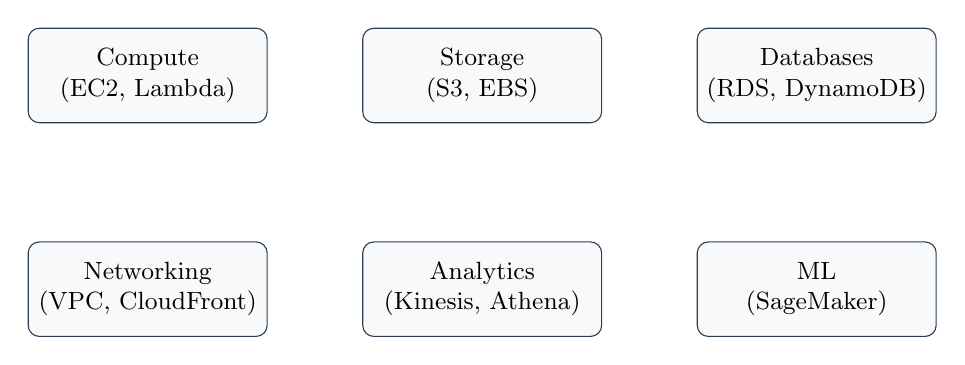
\begin{tikzpicture}[
                node distance=2.1cm,
                every node/.style={font=\small}
            ]
            \node[serviceBox] (compute) {Compute\\(EC2, Lambda)};
            \node[serviceBox, right=1.2cm of compute] (storage) {Storage\\(S3, EBS)};
            \node[serviceBox, right=1.2cm of storage] (db) {Databases\\(RDS, DynamoDB)};

            \node[serviceBox, below=1.5cm of compute] (network) {Networking\\(VPC, CloudFront)};
            \node[serviceBox, right=1.2cm of network] (analytics) {Analytics\\(Kinesis, Athena)};
            \node[serviceBox, right=1.2cm of analytics] (ml) {ML\\(SageMaker)};
        \end{tikzpicture}
    }
\end{center}

\clearpage

%--------------------------------------------------------------------
% 2. HOW COMPANIES USE AWS
%--------------------------------------------------------------------
\section{How Companies Use AWS}
\justifying

\subsection{Web Hosting}
Companies host static or dynamic websites on AWS. For example:
\begin{itemize}
    \item \textbf{Static content} on S3 + CloudFront
    \item \textbf{Dynamic apps} running on EC2 or containers
\end{itemize}

\vspace{-0.3cm}
\subsubsection{Static Site with S3 \& CloudFront}
\begin{center}
    \resizebox{\textwidth}{!}{%
        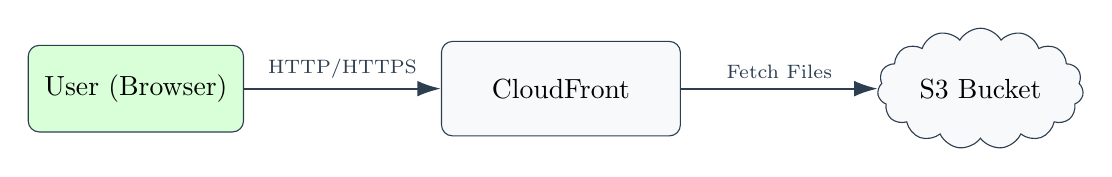
\begin{tikzpicture}[node distance=2.5cm]
            \node[userFigure] (user) {User (Browser)};
            \node[serviceBox, right=2.5cm of user] (cloudfront) {CloudFront};
            \node[cloudService, right=2.5cm of cloudfront] (s3) {S3 Bucket};

            \draw[arrowLine] (user) -- node[above]{\scriptsize HTTP/HTTPS} (cloudfront);
            \draw[arrowLine] (cloudfront) -- node[above]{\scriptsize Fetch Files} (s3);
        \end{tikzpicture}
    }
\end{center}

\subsection{Data Storage \& Backup}
\textbf{S3} is popular for storing large volumes of files (images, backups, logs) with high durability.

\subsection{Application Development}
Developers run code on:
\begin{itemize}
    \item \textbf{EC2} (full server control)
    \item \textbf{Lambda} (serverless, event-based)
\end{itemize}
And store data in \textbf{RDS} or \textbf{DynamoDB}.

\clearpage

%--------------------------------------------------------------------
% 3. HOW YOU CAN USE AWS
%--------------------------------------------------------------------
\section{How You Can Use AWS}
\justifying

\subsection{Start Small}
Try hosting a simple \textbf{static site on S3} or building a \textbf{file processor} where uploading an image to S3 triggers \textbf{Lambda} to resize it.

\subsection{Automate with Events}
Whenever a new file arrives in S3, a Lambda function can process it and then store metadata in a database.

\begin{center}
    \resizebox{\textwidth}{!}{%
        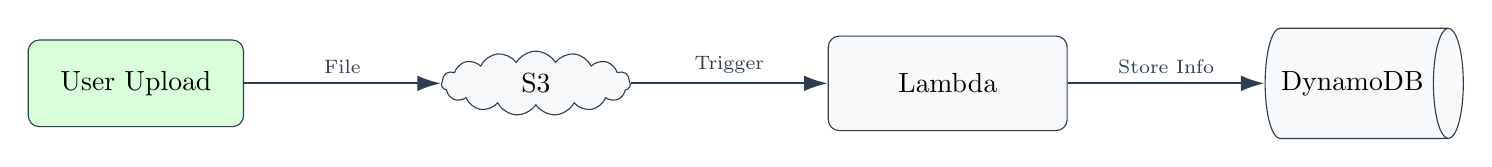
\begin{tikzpicture}[node distance=2.2cm]
            \node[userFigure] (upload) {User Upload};
            \node[cloudService, right=2.5cm of upload] (s3) {S3};
            \node[serviceBox, right=2.5cm of s3] (lambda) {Lambda};
            \node[database, right=2.5cm of lambda] (ddb) {DynamoDB};

            \draw[arrowLine] (upload) -- node[above]{\scriptsize File} (s3);
            \draw[arrowLine] (s3) -- node[above]{\scriptsize Trigger} (lambda);
            \draw[arrowLine] (lambda) -- node[above]{\scriptsize Store Info} (ddb);
        \end{tikzpicture}
    }
\end{center}

\subsection{Monitoring with CloudWatch}
\textbf{CloudWatch} gathers logs and metrics from your AWS resources. It can trigger alarms if your app needs scaling or if there’s an error spike.

\begin{center}
    \resizebox{0.9\textwidth}{!}{%
        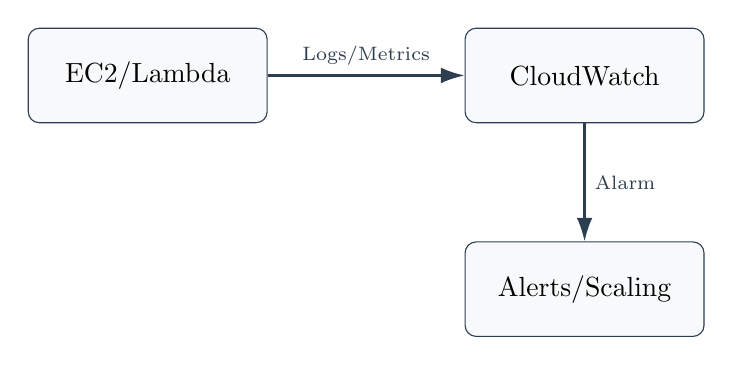
\begin{tikzpicture}[node distance=2.2cm]
            \node[serviceBox] (instances) {EC2/Lambda};
            \node[serviceBox, right=2.5cm of instances] (cw) {CloudWatch};

            \draw[arrowLine] (instances) -- node[above]{\scriptsize Logs/Metrics} (cw);

            \node[serviceBox, below=1.5cm of cw] (alert) {Alerts/Scaling};
            \draw[arrowLine] (cw) -- node[right]{\scriptsize Alarm} (alert);

        \end{tikzpicture}
    }
\end{center}

\clearpage

%--------------------------------------------------------------------
% 4. KEY AWS SERVICES (SIMPLIFIED)
%--------------------------------------------------------------------
\section{Key AWS Services (Simplified)}
\justifying

\subsection{S3 (Object Storage)}
Save files in “buckets.” Scalability and durability are built in.

\subsection{Lambda (Serverless Compute)}
Run code without managing servers. Write a function that triggers on events:

\begin{minted}[fontsize=\small, frame=single]{python}
def ProcessFile(event, context):
    S3_BUCKET_NAME = "my-bucket"
    fileKey = event["Records"][0]["s3"]["object"]["key"]
    # ... do something ...
    return {%
        "statusCode": 200,
        "body": "Processing complete"
    }
\end{minted}

\subsection{DynamoDB (NoSQL)}
A high-performance, key-value database. Great for session data, user profiles, or IoT data.

\subsection{EC2 (Virtual Servers)}
Manage your own virtual machines on AWS. Suitable for custom OS-level setups.

\subsection{CloudFront (CDN)}
Distribute content (images, videos, etc.) via a global network of edge locations, speeding up delivery.

\clearpage

%--------------------------------------------------------------------
% 5. HANDS-ON PROJECT IDEAS
%--------------------------------------------------------------------
\section{Hands-On Project Ideas}
\justifying

\subsection{Beginner}
\textbf{Static Website}: Host a personal portfolio on S3. Use CloudFront for global speed.
\textbf{File Processor}: Upload an image, trigger Lambda to transform it, store output in another S3 bucket.

\subsection{Intermediate}
\textbf{Web App (EC2 + RDS + S3)}: Backend on EC2, relational data in RDS, static files on S3.
\textbf{Serverless API (API Gateway + Lambda + DynamoDB)}: Create a REST or GraphQL endpoint without managing servers.

\subsection{Advanced}
\textbf{Real-Time Data (Kinesis + Lambda + DynamoDB)}: Stream data into Kinesis, process with Lambda, store results.
\textbf{Machine Learning (SageMaker + S3)}: Train a model with S3 data, deploy it for real-time predictions.

\clearpage

%--------------------------------------------------------------------
% 6. EXTRA VISUALS
%--------------------------------------------------------------------
\section{Extra Visuals}
\justifying

\subsection{A Typical Serverless Architecture}
\begin{center}
    \resizebox{\textwidth}{!}{%
        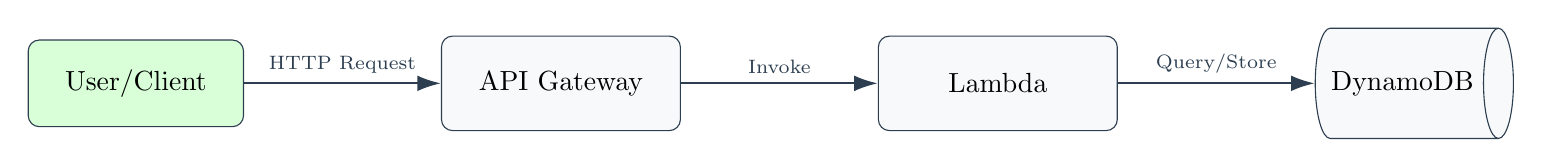
\begin{tikzpicture}[node distance=2.2cm]
            \node[userFigure] (user) {User/Client};
            \node[serviceBox, right=2.5cm of user] (apiGW) {API Gateway};
            \node[serviceBox, right=2.5cm of apiGW] (lambda) {Lambda};
            \node[database, right=2.5cm of lambda] (database) {DynamoDB};

            \draw[arrowLine] (user) -- node[above]{\scriptsize HTTP Request} (apiGW);
            \draw[arrowLine] (apiGW) -- node[above]{\scriptsize Invoke} (lambda);
            \draw[arrowLine] (lambda) -- node[above]{\scriptsize Query/Store} (database);
        \end{tikzpicture}
    }
\end{center}

\subsection{Monitoring Loop}
\begin{center}
    \resizebox{0.8\textwidth}{!}{%
        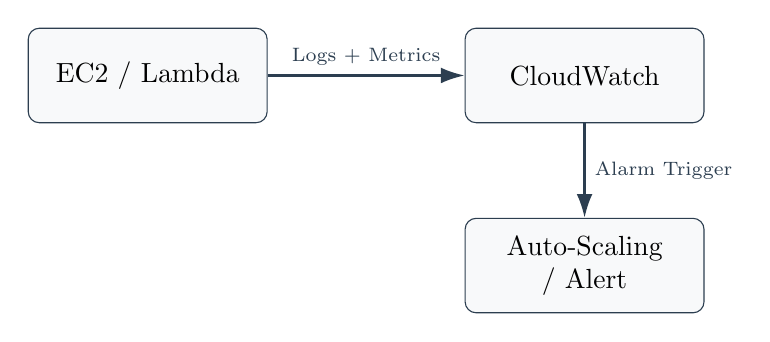
\begin{tikzpicture}[node distance=2.2cm]
            \node[serviceBox] (instances) {EC2 / Lambda};
            \node[serviceBox, right=2.5cm of instances] (cw) {CloudWatch};

            \draw[arrowLine] (instances) -- node[above]{\scriptsize Logs + Metrics} (cw);

            \node[serviceBox, below=1.2cm of cw] (scale) {Auto-Scaling / Alert};
            \draw[arrowLine] (cw) -- node[right]{\scriptsize Alarm Trigger} (scale);
        \end{tikzpicture}
    }
\end{center}

\clearpage

%--------------------------------------------------------------------
% 7. A LEARNING PATH
%--------------------------------------------------------------------
\section{A Learning Path}
\justifying

\subsection{1. Foundation}
\begin{itemize}
    \item \textbf{S3} for storage
    \item \textbf{Lambda} for event-driven code
    \item \textbf{DynamoDB} for simple NoSQL
\end{itemize}

\subsection{2. Intermediate Services}
\begin{itemize}
    \item \textbf{API Gateway} for REST/GraphQL
    \item \textbf{EC2} for custom server environments
    \item \textbf{RDS} for relational databases
\end{itemize}

\subsection{3. Advanced Tools}
\begin{itemize}
    \item \textbf{Kinesis} for streaming data
    \item \textbf{SageMaker} for ML
    \item \textbf{Athena/Redshift} for analytics
\end{itemize}

\begin{center}
    \resizebox{0.9\textwidth}{!}{%
        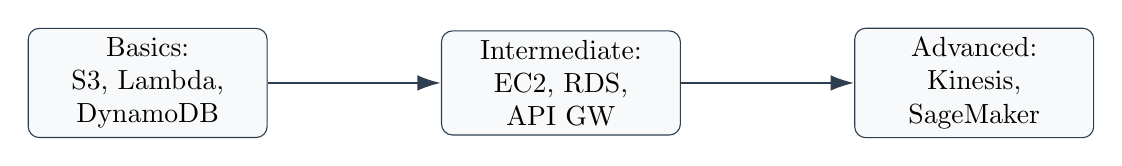
\begin{tikzpicture}[node distance=2.2cm]
            \node[serviceBox] (basic) {Basics:\\S3, Lambda, DynamoDB};
            \node[serviceBox, right=2.2cm of basic] (inter) {Intermediate:\\EC2, RDS, API GW};
            \node[serviceBox, right=2.2cm of inter] (advanced) {Advanced:\\Kinesis, SageMaker};

            \draw[arrowLine] (basic) -- (inter);
            \draw[arrowLine] (inter) -- (advanced);
        \end{tikzpicture}
    }
\end{center}

\clearpage

%--------------------------------------------------------------------
% CONCLUSION
%--------------------------------------------------------------------
\section*{Conclusion}
\addcontentsline{toc}{section}{Conclusion}
\justifying

By now, you should have a sense of how AWS can handle everything from simple websites to complex machine learning pipelines. Start with foundational services like \textbf{S3}, \textbf{Lambda}, and \textbf{DynamoDB}, then move on to \textbf{EC2}, \textbf{RDS}, and beyond. If you need real-time data or ML solutions, \textbf{Kinesis} and \textbf{SageMaker} are waiting.

\textbf{Key tips}:
\begin{itemize}
    \item Use the \textbf{AWS Free Tier} to experiment cheaply.
    \item Build real, small-scale projects to gain confidence.
    \item Check out the
          \href{https://aws.amazon.com/documentation/}{\textbf{official AWS docs}}
          for deeper dives on each service.
\end{itemize}

\textbf{Happy Building!}

\end{document}
